\section{Methodology}
The overall approach includes Feature Engineering, Model Training, Stacking and F1-Maximization as shown 
in Figure~\ref{fig:Approach}.
We treat each consumer-item as an individual object and generate weekly time series based on historical transaction for 
each object. The target value at each time step (week) takes a binary input, 1/0 (purchased/not purchased).
We then generate various types of features including datetime related, label encoded and target encoded 
within and across objects. Below are the feature groups with the type of features within each group:
\begin{itemize}
\item {\bf Datetime:} Weekday order split of the shopper and the item, daypart order split of the item, Proportion of 
repurchase in previous orders, number of times A bought B in n recent orders and multiple interactions of 
user-item related features.
\item {\bf Consumer Profile:} Total number of orders by the user, Number of distinct items ordered by the user
Time since first order by the shopper, Time since last order by the shopper, Averge time gap between orders
Reorder rate of the user, Reorder frequency of the user, Time of the day user visits, Specific item ordered by user in the past
Order size based features, Orders with no previously reordered item
\item {\bf Item Profile:} Time since first order for the merchandise, Time since last order for the merchandise
Averge time gap between orders, Reorder rate of the item, Reorder frequency of the item
Number of co-occuring items with this item, Item's average position in the cart, Statistics around order streak for this item
Item's total number of orders, Number of distinct users, Number of users buying it as one shot item
\item {\bf Consumer-Item Profile:} Time since first order for each combination, Time since last order for each combination
Averge time gap between orders, Reorder rate of the combination, Reorder frequency of the combination, 
Streak -user purchased the item in a row, Average position in the cart, Co-occurance Statistics
Replacement items, Total number of orders for the combination, If user already ordered the item today
\end{itemize}
The model we needed to build, thus, should learn to identify similarly behaving time series across latent
parameters, and also take into account consumer and item variations in comparing the time series.
A point in a time series is represented
  \begin{equation}
    \begin{array}{l}
      y\textsubscript{(C\textsubscript{t},I\textsubscript{t})}  = f((IA\textsubscript{t}),(CA\textsubscript{t},.., CA\textsubscript{t-n}),
      (CIA\textsubscript{t},.., CIA\textsubscript{t-n}), \\
      (D\textsubscript{t},.., D\textsubscript{t-n}))
    \end{array}
  \end{equation}
where yit is sales for item ’i’ at time ’t’, Ai is attribute of the item ’i’ like colour - blue, material - cotton etc., 
Mit indicate merchandising factors like discount, promotion for items ’i’ at time ’t’, Dit are derived features like 
trend, seasonality which are inferred from data and affect the sales, p is number of time lag.

%\begin{figure}[t]
%  \centering 
%  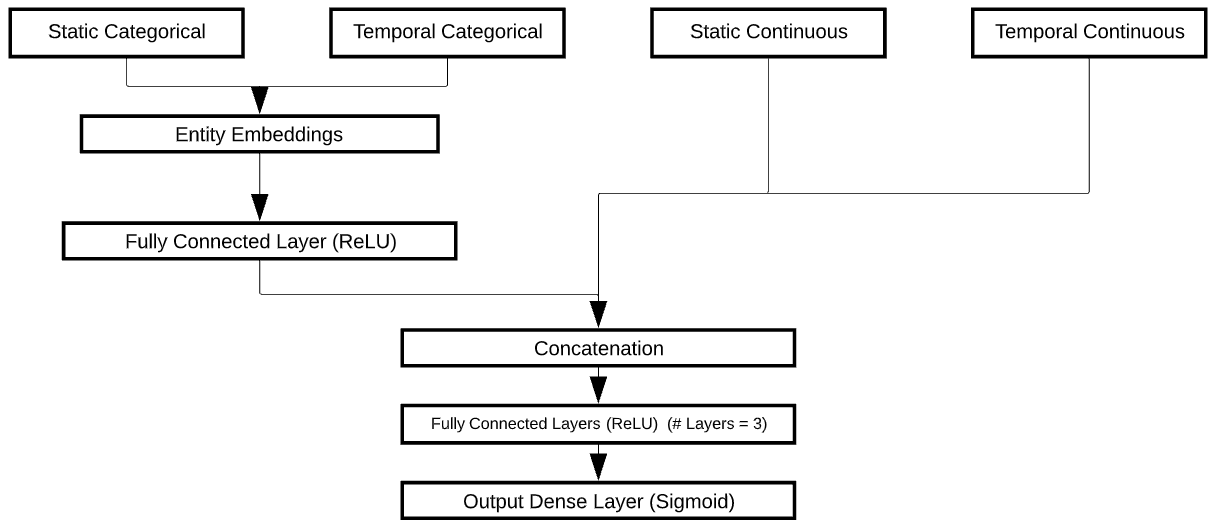
\includegraphics[width=3.3in]{img/MLP.png} 
%  \caption{Overall Approach} 
%  \label{fig:Approach} 
%\end{figure}

\subsection{Accuracy Measure}
Consumer Basket prediction framework should be able to strike good balance between Precision and Recall. 
Precision refers to the ratio of number of predicted items actually purchased from the predicted items, 
\[Precision = \frac{True Positive} {True Positive + False Positive}\]
whereas Recall refers to the ratio of predicted items actually purchased from the items in the actual basket. 
\[Recall = \frac{True Positive} {True Positive + False Negative}\]
F1 Score is needed when you want to seek a balance between Precision and Recall.
We have previously seen that accuracy can be largely contributed by a large number of True Negatives which 
in most business circumstances, we do not focus on much whereas False Negative and False Positive usually has 
business costs, thus F1 Score might be a better measure to use if we need to seek a balance
between Precision and Recall and there is an uneven class distribution (large number of Actual Negatives).
\[F1-Score = \frac{2 * Precision * Recall} {Precision + Recall}\]

\subsection{Model Architectures}
As mentioned in previous section, traditional time series models are not suitable choice for f . Hence, we work with machine learning models ranging from tree based models like Random Forest
and various flavours of Gradient Boosted Trees, to deep learning
models. We train two deep learning models, first of which uses
Multi Layer Perceptron (MLP) architecture, and second is based
on LSTM (chosen due to its ability to model long term temporal
dependencies), to derive the relation

